\chapter{Range Minimum Queries}

Eine \term{range minimum Query}\index{range minimum query} gibt für ein array \( A \) (\( \left\vert A \right\vert \eqqcolon n \)) die Position des kleinsten Elements zwischen zwei Begrenzern \( 1 \leq \bm{l} < \bm{r} \leq n \) zurück:
\begin{equation*}
  \text{rmq}_A(l,r) = (\text{arg})\min_{l \leq k \leq r}A[k]
\end{equation*}

\begin{figure}[H]
  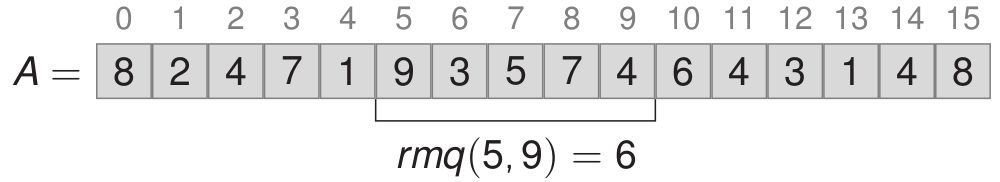
\includegraphics[width=0.6\textwidth]{rmqExample}
  \caption{Beispiel einer range minimum query}
\end{figure}

Ein naiver Ansatz, um eine range minimum query auszuführen, ist, einfach das Array zu durchlaufen und das Minimum zu speichern (und wenn nötig zu aktualisieren). Dafür ist keine Vorbereitungsarbeit nötig (also \( O(1) \)) und die Abfrage ist in \( O(n) \). Wir notieren
\begin{equation*}
  \left\langle O(1), O(n) \right\rangle\text{.}
\end{equation*}

\subsection{Lösung 1 --- \( \left\langle O(n), O(\log n) \right\rangle \)}

Baut man einen binären Suchbaum über das Array auf, so lässt sich die Komplexität der Abfrage auf \( O(\log n) \) reduzieren.

Hierzu betrachtet man die größtmöglichen Knoten, die vollständig im Abfrageintervall liegen (grün dargestellt), und berechnet das Minimum dieser.

\begin{figure}[H]
  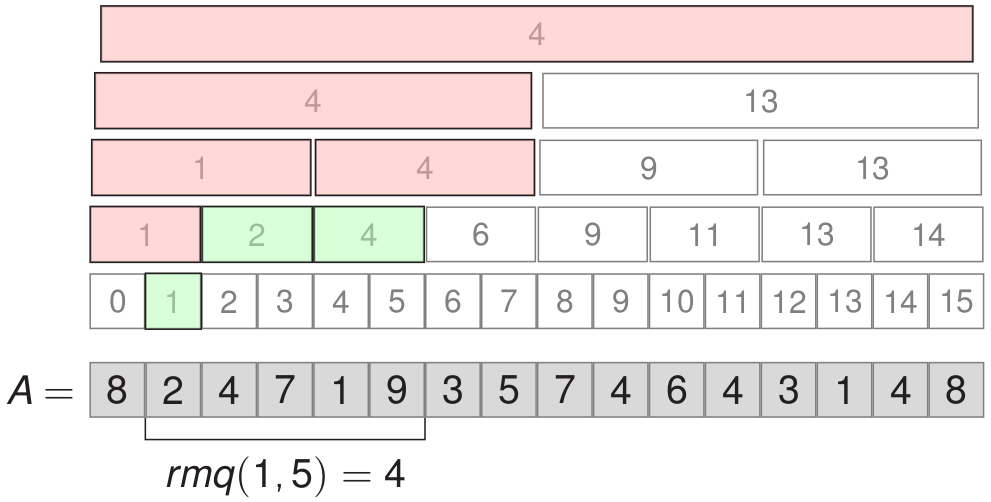
\includegraphics[width=0.6\textwidth]{rmqBST}
  \caption{Die grauen Felder stellen die Knoten des binären Suchbaums dar, sie beinhalten die Position des Arrays, an der der Teilbaum, dessen Wurzel sie sind, den minimalen Wert annimmt. Die größten Knoten, die vollständig im Intervall liegen, sind grün markiert.}
\end{figure}

\subsection{Lösung 2 --- \( \left\langle O(n\log n),O(1) \right\rangle \)}

Wir reduzieren nun die Zeit, die zum Bearbeiten der rmq benötigt wird, auf \( O(1) \), indem wir für jedes \( A[i] \) ein Array \( M_i[0,\log n] \) vorberechnen. Es sei
\begin{equation*}
  M_i[j] = \text{rmq}_A(i,i+2^j-1)\text{.}
\end{equation*}

Idee ist es nun, \( \text{rmq}_A(l,r) \) aus der Überdeckung des Intervalls durch zwei Zweierpotenzen zu berechnen.

Wir suchen dafür \( 2^{\lfloor l - r \rfloor} \), also die größte Zweierpotenz, die kleiner ist als die Länge des Intervalls. Offensichtlich ist diese Zweierpotenz mehr als halb so groß wie das Intervall, also ist \( \text{rmq}_A(l,r) \) entweder das Minimum der ersten oder zweiten überdeckenden Zweierpotenz.

\begin{figure}[H]
  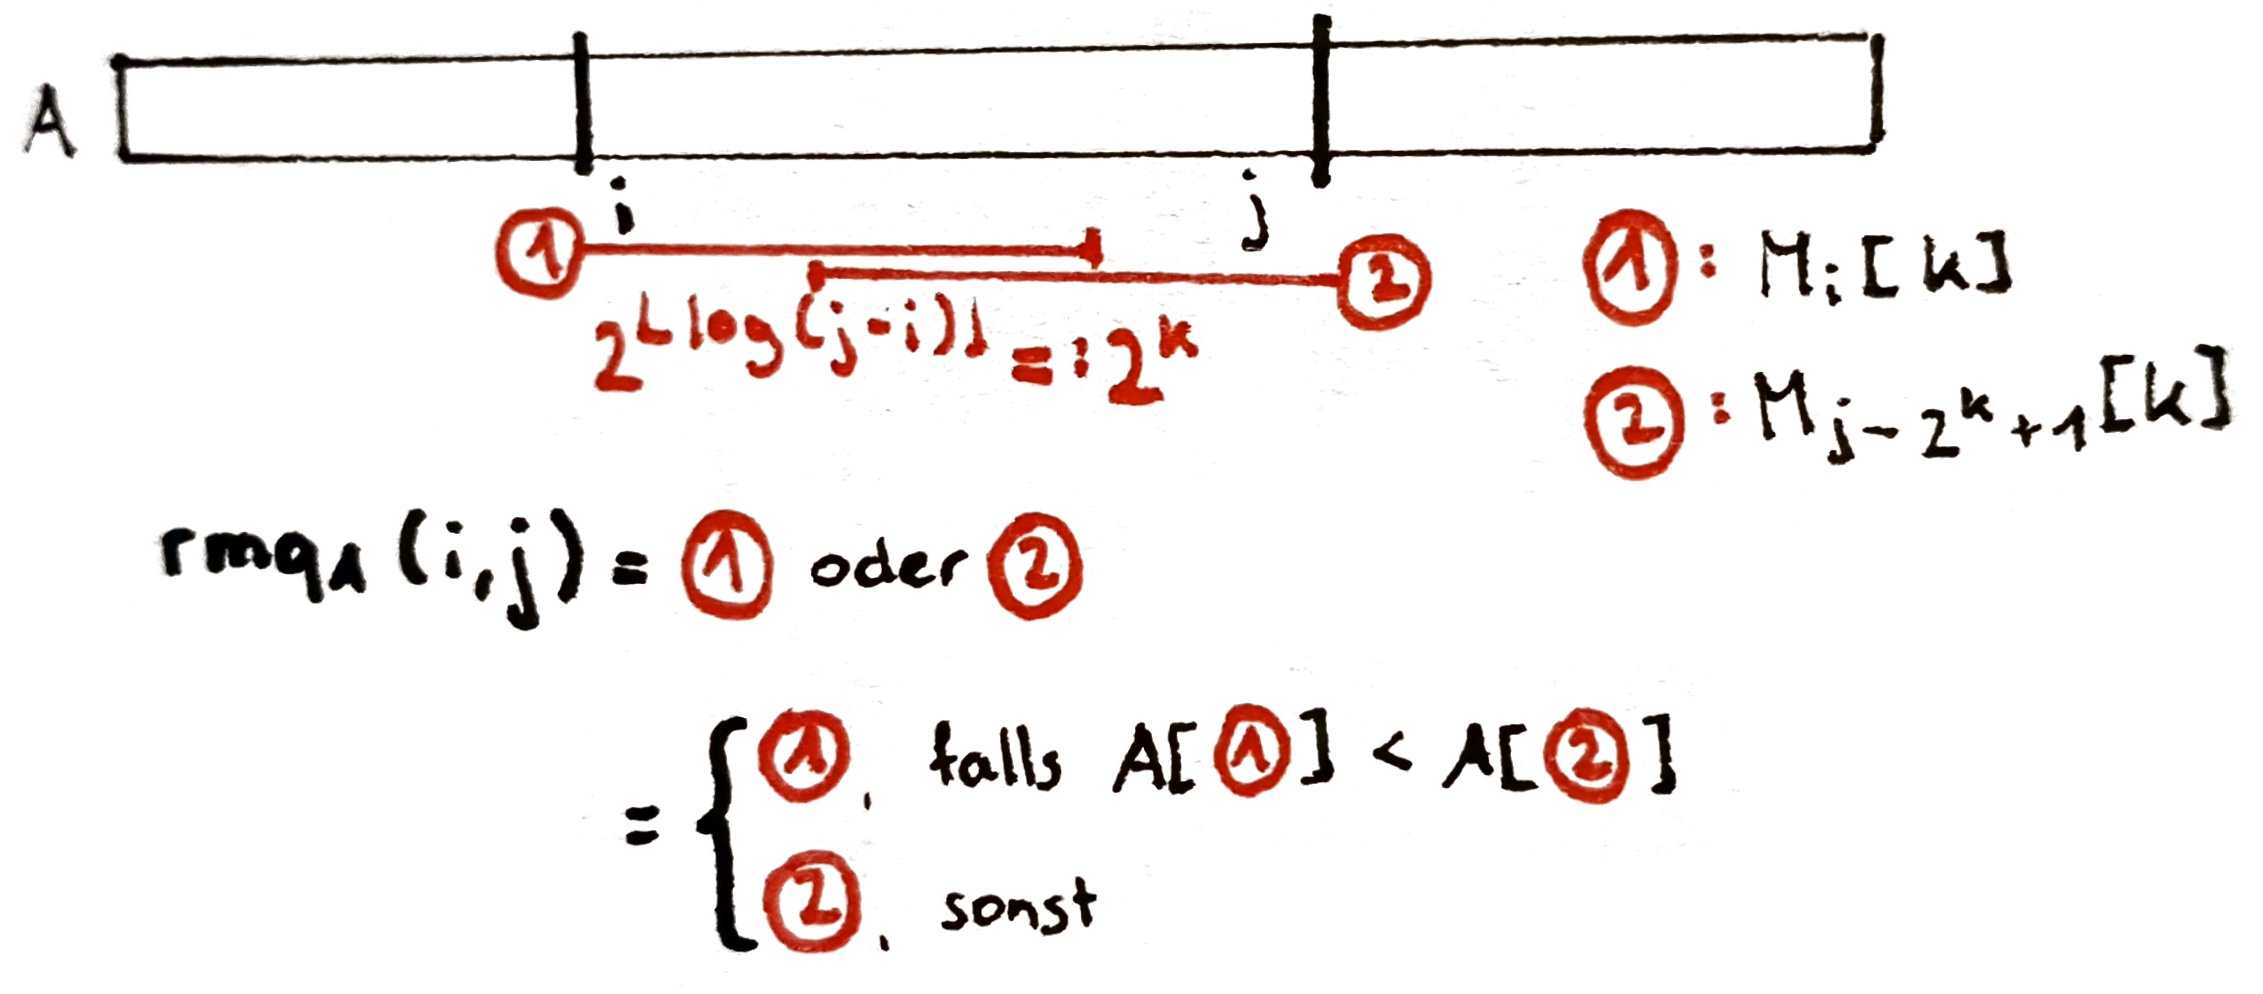
\includegraphics[width=0.6\textwidth]{rmqVersion2}
  \caption{Funktionsweise des zweiten rmq-Algorithmus}
\end{figure}

\subsection{Lösung 3 --- \( \left\langle O(n \log \log n), O(1) \right\rangle \)}

Wir wenden folgende Prozedur an:

\begin{enumerate}
  \item \( A \) in \( t = \frac{n}{\log n} \) Blöcke \( B_0, \dots, B_{t-1} \) der Größe \( \log n \) unterteilen.
  \item Array \( S[0,t-1] \) mit \( S[i] = \min\left \{ x \in B_i \right \} \) erstellen, rmq-Struktur nach Lösung 2 für \( S \) berechnen.
  \item Für jeden Block \( B_i \) rmq-Struktur nach Lösung 2 berechnen.
\end{enumerate}

Diese Prozedur liegt in \( O(n \log \log n) \).

Soll nun \( \text{rmq}_A(l,r) \) bestimmt werden, so geht das folgendermaßen:

\begin{enumerate}
  \item Bestimme die Blöcke \( l \in B_{l'} \) und \( r \in B_{r'} \).
  \item Berechne \( m = \text{rmq}_S(l'+1, r'-1) \). Wir nutzen also die Struktur über \( S \), um die rmq-Werte der Blöcke zwischen den beiden Grenzblöcken zu berechnen.
  \item Es seien \( k_0,k_1,k_2 \) die \( \text{rmq}_A \)-Resultate in den Blöcken \( l' \), \( r' \) und \( m \)
  \item \( \text{rmq}_A(l,r) = \text{arg}\min \left \{ A[k_0],A[k_1],A[k_2] \right \} \)\text{.}
\end{enumerate}